\chapter{Tree Data Structures}

\section{Introduction}
A \textbf{tree} is a hierarchical data structure that consists of nodes connected by edges. Trees are widely used in computer science to represent hierarchical relationships such as file systems, organizational structures, and decision processes. A \textbf{binary tree} is a tree in which each node has at most two children, commonly referred to as the left and right child. A \textbf{binary search tree (BST)} is a special kind of binary tree that maintains an order: for any node, all elements in its left subtree are less than or equal to the node's key and all elements in its right subtree are greater.

\section{Definition, Terminology, and Formulas}
\subsection{Basic Definitions and Terminology}
A tree \( T \) is defined as a pair \( (V, E) \) where:
\begin{itemize}
    \item \( V \) is a set of nodes.
    \item \( E \) is a set of edges connecting the nodes.
\end{itemize}
Key terms include:
\begin{description}
    \item[Root:] The topmost node in a tree.
    \item[Parent:] A node that has one or more children.
    \item[Child:] A node that is a descendant of another node.
    \item[Leaf:] A node with no children.
    \item[Subtree:] A tree consisting of a node and its descendants.
    \item[Height:] The length of the longest path from the root to a leaf. Formally, for a node \( v \), 
    \[
    \text{height}(v) = \begin{cases} 
    0, & \text{if } v \text{ is a leaf,} \\
    1 + \max(\text{height}(v.\text{left}), \text{height}(v.\text{right})), & \text{otherwise.}
    \end{cases}
    \]
    \item[Depth:] The length of the path from the root to the node.
\end{description}

\subsection{Performance Formulas}
For a balanced binary tree containing \( n \) nodes:
\begin{itemize}
    \item \textbf{Search, Insertion, Deletion:} Average time complexity is \( O(\log n) \).
\end{itemize}
In a degenerate (unbalanced) tree, these operations degrade to \( O(n) \).

\subsection{Summary Table of Tree Properties}
\begin{table}[h!]
\centering
\small
\begin{tabular}{p{3.5cm} p{3cm} p{4cm} p{3cm}}
\toprule
\textbf{Tree Type} & \textbf{Average Height} & \textbf{Search / Insertion / Deletion} & \textbf{Space Complexity} \\
\midrule
Binary Search Tree (Balanced)   & \( O(\log n) \) & \( O(\log n) \) & \( O(n) \) \\
Binary Search Tree (Unbalanced) & \( O(n) \)      & \( O(n) \)      & \( O(n) \) \\
AVL Tree / Red-Black Tree       & \( O(\log n) \) & \( O(\log n) \) & \( O(n) \) \\
Complete Binary Tree            & \( O(\log n) \) & \( O(\log n) \) & \( O(n) \) \\
\bottomrule
\end{tabular}
\caption{Comparison of Tree Data Structures}
\label{tab:tree-comparison}
\normalsize
\end{table}





\section{Types of Tree Data Structures}
Trees come in many forms, each with its own characteristics:
\begin{itemize}
    \item \textbf{Binary Tree}: Each node has at most two children.
    \item \textbf{Binary Search Tree (BST)}: A binary tree that maintains sorted order.
    \item \textbf{Balanced Trees}: Such as AVL trees and Red-Black trees, which maintain \( O(\log n) \) height.
    \item \textbf{Complete Binary Tree}: A binary tree in which all levels, except possibly the last, are completely filled.
    \item \textbf{Heap}: A specialized tree-based structure that satisfies the heap property (used for priority queues).
    \item \textbf{B-tree and B+ tree}: Used in databases and filesystems, designed to work well on disks.
    \item \textbf{Trie}: A tree used for storing associative arrays where the keys are usually strings.
\end{itemize}

\section{Converting Arrays into Trees}
A common example is converting an array into a \textbf{complete binary tree}. If we have an array \( A \) with \( n \) elements, we can represent it as a complete binary tree where:
\begin{itemize}
    \item The element at index \( i \) is the parent.
    \item The left child is at index \( 2i+1 \).
    \item The right child is at index \( 2i+2 \).
\end{itemize}
This representation is particularly efficient because it uses the array indices to simulate pointers, which is common in heap implementations.

\section{Diagrams of Tree Structures and Traversals}
\subsection{Binary Tree Diagram}
The diagram below shows a simple binary tree:

\begin{center}
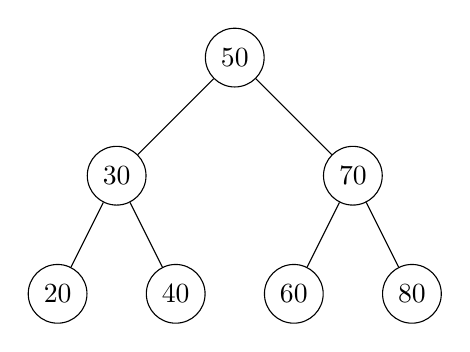
\begin{tikzpicture}[level distance=1.5cm,
  level 1/.style={sibling distance=3cm},
  level 2/.style={sibling distance=1.5cm}]
  \node [draw, circle] {50}
    child { node [draw, circle] {30}
      child { node [draw, circle] {20} }
      child { node [draw, circle] {40} }
    }
    child { node [draw, circle] {70}
      child { node [draw, circle] {60} }
      child { node [draw, circle] {80} }
    };
\end{tikzpicture}
\end{center}

\subsection{Traversal Order Example}
For the tree above:
\begin{itemize}
    \item \textbf{Preorder}: 50, 30, 20, 40, 70, 60, 80
    \item \textbf{Inorder}: 20, 30, 40, 50, 60, 70, 80
    \item \textbf{Postorder}: 20, 40, 30, 60, 80, 70, 50
    \item \textbf{Level Order}: 50, 30, 70, 20, 40, 60, 80
\end{itemize}

\section{C++ Implementation of a Binary Search Tree}
Below is a complete C++ implementation of a binary search tree (BST) including insertion, search, deletion, and all traversal methods.

\begin{lstlisting}[caption={C++ implementation of a Binary Search Tree}]
#include <iostream>
#include <queue>
using namespace std;

struct Node {
    int key;
    Node* left;
    Node* right;
    Node(int key) : key(key), left(nullptr), right(nullptr) {}
};

class BST {
private:
    Node* root;
    
    Node* insert(Node* node, int key) {
        if (node == nullptr)
            return new Node(key);
        if (key < node->key)
            node->left = insert(node->left, key);
        else if (key > node->key)
            node->right = insert(node->right, key);
        return node;
    }
    
    Node* search(Node* node, int key) {
        if (node == nullptr || node->key == key)
            return node;
        if (key < node->key)
            return search(node->left, key);
        else
            return search(node->right, key);
    }
    
    // Find the minimum node in a subtree
    Node* minValueNode(Node* node) {
        Node* current = node;
        while (current && current->left != nullptr)
            current = current->left;
        return current;
    }
    
    Node* remove(Node* node, int key) {
        if (node == nullptr) return node;
        if (key < node->key)
            node->left = remove(node->left, key);
        else if (key > node->key)
            node->right = remove(node->right, key);
        else {
            // Node with only one child or no child
            if (node->left == nullptr) {
                Node* temp = node->right;
                delete node;
                return temp;
            } else if (node->right == nullptr) {
                Node* temp = node->left;
                delete node;
                return temp;
            }
            // Node with two children: Get the inorder successor (smallest in the right subtree)
            Node* temp = minValueNode(node->right);
            node->key = temp->key;
            node->right = remove(node->right, temp->key);
        }
        return node;
    }
    
    // Preorder Traversal (Root, Left, Right)
    void preorder(Node* node) {
        if (node != nullptr) {
            cout << node->key << " ";
            preorder(node->left);
            preorder(node->right);
        }
    }
    
    // Inorder Traversal (Left, Root, Right)
    void inorder(Node* node) {
        if (node != nullptr) {
            inorder(node->left);
            cout << node->key << " ";
            inorder(node->right);
        }
    }
    
    // Postorder Traversal (Left, Right, Root)
    void postorder(Node* node) {
        if (node != nullptr) {
            postorder(node->left);
            postorder(node->right);
            cout << node->key << " ";
        }
    }
    
public:
    BST() : root(nullptr) {}
    
    void insert(int key) {
        root = insert(root, key);
    }
    
    Node* search(int key) {
        return search(root, key);
    }
    
    void remove(int key) {
        root = remove(root, key);
    }
    
    void preorder() {
        preorder(root);
        cout << "\n";
    }
    
    void inorder() {
        inorder(root);
        cout << "\n";
    }
    
    void postorder() {
        postorder(root);
        cout << "\n";
    }
    
    // Level Order Traversal (Breadth-first)
    void levelOrder() {
        if (root == nullptr) return;
        queue<Node*> q;
        q.push(root);
        while (!q.empty()) {
            Node* current = q.front();
            q.pop();
            cout << current->key << " ";
            if (current->left != nullptr)
                q.push(current->left);
            if (current->right != nullptr)
                q.push(current->right);
        }
        cout << "\n";
    }
};

int main() {
    BST tree;
    // Insertion
    tree.insert(50);
    tree.insert(30);
    tree.insert(20);
    tree.insert(40);
    tree.insert(70);
    tree.insert(60);
    tree.insert(80);
    
    cout << "Inorder Traversal: ";
    tree.inorder();      // 20 30 40 50 60 70 80
    
    cout << "Preorder Traversal: ";
    tree.preorder();     // 50 30 20 40 70 60 80
    
    cout << "Postorder Traversal: ";
    tree.postorder();    // 20 40 30 60 80 70 50
    
    cout << "Level Order Traversal: ";
    tree.levelOrder();   // 50 30 70 20 40 60 80
    
    // Search for a key
    int searchKey = 40;
    if (tree.search(searchKey))
        cout << "Key " << searchKey << " found in the tree.\n";
    else
        cout << "Key " << searchKey << " not found in the tree.\n";
    
    // Deletion
    tree.remove(30);
    cout << "Inorder Traversal after deleting 30: ";
    tree.inorder();
    
    return 0;
}
\end{lstlisting}

\section{AVL Trees: Implementation and Rotations}
AVL trees are a type of self-balancing binary search tree that ensures the difference in heights (balance factor) between the left and right subtrees for any node is at most one. This guarantees \( O(\log n) \) time complexity for search, insertion, and deletion.

\subsection{Node Structure and Balance Factor}
For an AVL tree, each node is augmented with a \textbf{height} attribute. The \textbf{balance factor} is defined as:
\[
\text{Balance Factor} = \text{height(left subtree)} - \text{height(right subtree)}
\]
A node is balanced if its balance factor is \(-1\), \(0\), or \(1\).

\subsection{AVL Rotations}
To restore balance after an insertion or deletion, AVL trees perform rotations:
\begin{itemize}
    \item \textbf{Right Rotation}: Used for a left-left imbalance.
    \item \textbf{Left Rotation}: Used for a right-right imbalance.
    \item \textbf{Left-Right Rotation}: A left rotation followed by a right rotation, used for a left-right imbalance.
    \item \textbf{Right-Left Rotation}: A right rotation followed by a left rotation, used for a right-left imbalance.
\end{itemize}

\subsection{Diagram: Left Rotation Example}
Before rotation (inserting keys causing a right-right imbalance):
\begin{center}
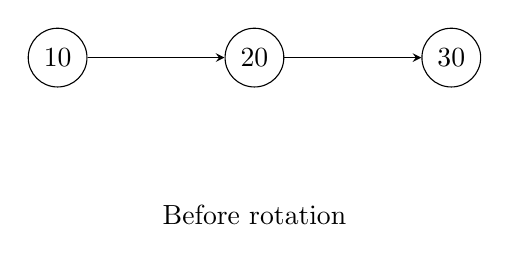
\begin{tikzpicture}[>=stealth, node distance=1.5cm]
    \node[draw, circle] (x) {10};
    \node[draw, circle, right of=x, xshift=1cm] (y) {20};
    \node[draw, circle, right of=y, xshift=1cm] (z) {30};
    \draw[->] (x) -- (y);
    \draw[->] (y) -- (z);
    \node[below of=y, yshift=-0.5cm] {Before rotation};
\end{tikzpicture}
\end{center}

After performing a left rotation at node 10, the tree becomes:
\begin{center}
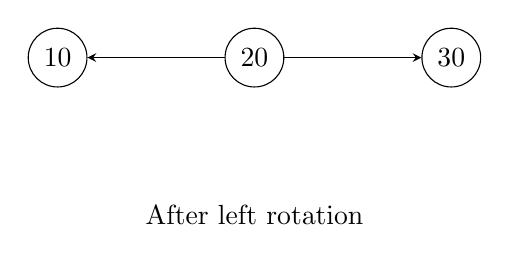
\begin{tikzpicture}[>=stealth, node distance=1.5cm]
    \node[draw, circle] (y) {20};
    \node[draw, circle, left of=y, xshift=-1cm] (x) {10};
    \node[draw, circle, right of=y, xshift=1cm] (z) {30};
    \draw[->] (y) -- (x);
    \draw[->] (y) -- (z);
    \node[below of=y, yshift=-0.5cm] {After left rotation};
\end{tikzpicture}
\end{center}

\subsection{C++ Implementation of an AVL Tree}
Below is a complete C++ implementation for an AVL tree that includes node structure, insertion with rebalancing (rotations), and a preorder traversal function for demonstration.

\begin{lstlisting}[caption={C++ implementation of an AVL Tree}]
#include <iostream>
#include <algorithm>
using namespace std;

struct AVLNode {
    int key;
    int height;
    AVLNode *left, *right;
    AVLNode(int key) : key(key), height(1), left(nullptr), right(nullptr) {}
};

int height(AVLNode *node) {
    return node ? node->height : 0;
}

int getBalance(AVLNode *node) {
    return node ? height(node->left) - height(node->right) : 0;
}

AVLNode* rightRotate(AVLNode* y) {
    AVLNode *x = y->left;
    AVLNode *T2 = x->right;
    // Perform rotation
    x->right = y;
    y->left = T2;
    // Update heights
    y->height = max(height(y->left), height(y->right)) + 1;
    x->height = max(height(x->left), height(x->right)) + 1;
    return x;
}

AVLNode* leftRotate(AVLNode* x) {
    AVLNode *y = x->right;
    AVLNode *T2 = y->left;
    // Perform rotation
    y->left = x;
    x->right = T2;
    // Update heights
    x->height = max(height(x->left), height(x->right)) + 1;
    y->height = max(height(y->left), height(y->right)) + 1;
    return y;
}

AVLNode* insert(AVLNode* node, int key) {
    // Standard BST insertion
    if(!node)
       return new AVLNode(key);
    if(key < node->key)
       node->left = insert(node->left, key);
    else if(key > node->key)
       node->right = insert(node->right, key);
    else
       return node; // no duplicates allowed

    // Update the height of this ancestor node
    node->height = max(height(node->left), height(node->right)) + 1;
    int balance = getBalance(node);

    // Left Left Case
    if(balance > 1 && key < node->left->key)
        return rightRotate(node);
    // Right Right Case
    if(balance < -1 && key > node->right->key)
        return leftRotate(node);
    // Left Right Case
    if(balance > 1 && key > node->left->key) {
        node->left = leftRotate(node->left);
        return rightRotate(node);
    }
    // Right Left Case
    if(balance < -1 && key < node->right->key) {
        node->right = rightRotate(node->right);
        return leftRotate(node);
    }
    return node;
}

void preOrder(AVLNode *root) {
    if(root != nullptr) {
        cout << root->key << " ";
        preOrder(root->left);
        preOrder(root->right);
    }
}

int main() {
    AVLNode *root = nullptr;
    int arr[] = {10, 20, 30, 40, 50, 25};
    for (int i = 0; i < 6; i++)
        root = insert(root, arr[i]);
    cout << "Preorder traversal of the constructed AVL tree is: \n";
    preOrder(root);
    return 0;
}
\end{lstlisting}

\section{AVL Trees: Rotations}

AVL trees are a type of self-balancing binary search tree that ensures the difference in heights (balance factor) between the left and right subtrees for any node is at most one. This guarantees \( O(\log n) \) time complexity for search, insertion, and deletion.

\subsection{Node Structure and Balance Factor}
For an AVL tree, each node is augmented with a \textbf{height} attribute. The \textbf{balance factor} of a node is defined as:
\[
\text{Balance Factor} = \text{height(left subtree)} - \text{height(right subtree)}
\]
A node is balanced if its balance factor is \(-1\), \(0\), or \(1\).

\subsection{AVL Rotations: Terminology and Diagrams}
When an insertion or deletion causes a node's balance factor to fall outside of \([-1, 1]\), the AVL tree must be rebalanced using rotations. The key rotation types are:

\begin{itemize}
    \item \textbf{Right Rotation}: Corrects a left-left imbalance.
    \item \textbf{Left Rotation}: Corrects a right-right imbalance.
    \item \textbf{Left-Right Rotation}: A combination; perform a left rotation on the left child, then a right rotation on the node.
    \item \textbf{Right-Left Rotation}: A combination; perform a right rotation on the right child, then a left rotation on the node.
\end{itemize}

\subsubsection{Right Rotation Diagram}
\textbf{Right Rotation} is used when a node's left subtree is heavy (i.e., a left-left imbalance). Consider the following subtree:

\textbf{Before right rotation:}
\begin{center}
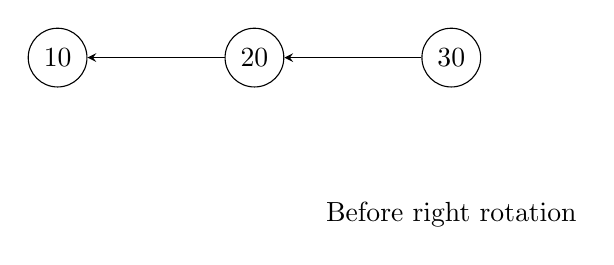
\begin{tikzpicture}[>=stealth, node distance=1.5cm]
    \node[draw, circle] (y) {30};
    \node[draw, circle, left of=y, xshift=-1cm] (x) {20};
    \node[draw, circle, left of=x, xshift=-1cm] (T1) {10};
    \draw[->] (x) -- (T1);
    \draw[->] (y) -- (x);
    \node[below of=y, yshift=-0.5cm] {Before right rotation};
\end{tikzpicture}
\end{center}

\textbf{After right rotation at node \(y\):}
\begin{center}
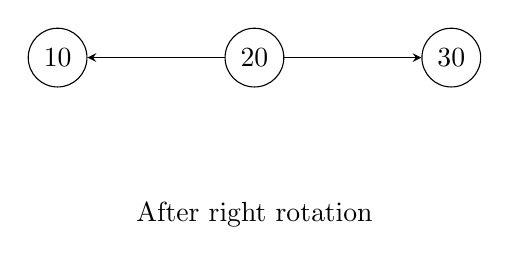
\begin{tikzpicture}[>=stealth, node distance=1.5cm]
    \node[draw, circle] (x) {20};
    \node[draw, circle, right of=x, xshift=1cm] (y) {30};
    \node[draw, circle, left of=x, xshift=-1cm] (T1) {10};
    \draw[->] (x) -- (T1);
    \draw[->] (x) -- (y);
    \node[below of=x, yshift=-0.5cm] {After right rotation};
\end{tikzpicture}
\end{center}

\subsubsection{Left Rotation Diagram}
\textbf{Left Rotation} is used when a node's right subtree is heavy (i.e., a right-right imbalance). Consider the following subtree:

\textbf{Before left rotation:}
\begin{center}
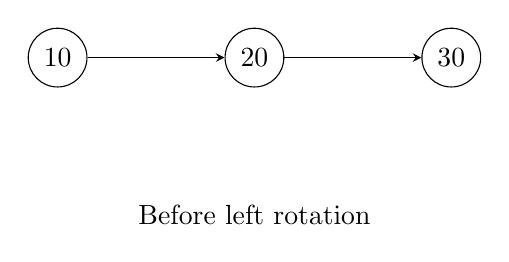
\begin{tikzpicture}[>=stealth, node distance=1.5cm]
    \node[draw, circle] (x) {10};
    \node[draw, circle, right of=x, xshift=1cm] (y) {20};
    \node[draw, circle, right of=y, xshift=1cm] (z) {30};
    \draw[->] (x) -- (y);
    \draw[->] (y) -- (z);
    \node[below of=y, yshift=-0.5cm] {Before left rotation};
\end{tikzpicture}
\end{center}

\textbf{After left rotation at node \(x\):}
\begin{center}
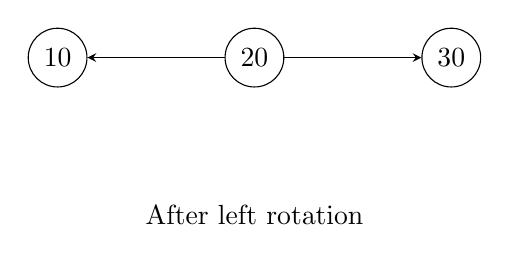
\begin{tikzpicture}[>=stealth, node distance=1.5cm]
    \node[draw, circle] (y) {20};
    \node[draw, circle, left of=y, xshift=-1cm] (x) {10};
    \node[draw, circle, right of=y, xshift=1cm] (z) {30};
    \draw[->] (y) -- (x);
    \draw[->] (y) -- (z);
    \node[below of=y, yshift=-0.5cm] {After left rotation};
\end{tikzpicture}
\end{center}

\section{Conclusion}
This chapter has provided an in-depth exploration of tree data structures. We began with the theoretical foundations and key terminology, introduced essential formulas, and presented a summary table of tree properties. We then discussed various types of trees—including binary trees, binary search trees, balanced trees, heaps, and tries—and explained how to convert an array into a complete binary tree.